\documentclass[11pt,spanish]{article}
\usepackage[utf8]{inputenc}
\usepackage{babel}
\usepackage{fullpage}
\usepackage{listings}
\usepackage{mathpazo}
\usepackage{enumitem}
\usepackage{courier}
\usepackage{xcolor}
\usepackage{textcomp}
\usepackage{amsmath}
\usepackage{amssymb}
\usepackage{tikz}
\usepackage{fancyhdr}
\usepackage{graphics}

\newcommand{\titulo}{Certamen 1 tipo (versión 2)}
\newcommand{\cc}[1]{\hfil\texttt{#1}\hfil}

\pagestyle{fancy}
\lhead{%
  {\Large\bfseries Programación---\titulo} \\
  Nombre: \nombre\hfill
  Rol:    \rol
  \vspace{2ex}
}
\chead{}\rhead{}\lfoot{}\cfoot{}\rfoot{}
\renewcommand{\headrulewidth}{0pt}
\addtolength{\headheight}{7ex}
\headsep=4ex


\newcommand{\onelinerule}{\rule[2.3ex]{0pt}{0pt}}
\newcommand{\twolinerule}{\rule[6.2ex]{0pt}{0pt}}
\newcommand{\respuesta}{\framebox[\textwidth]{\twolinerule}}
\newcommand{\nombre}{%
  \begin{tikzpicture}[xscale=.4,yscale=.7]
    \draw (0, 0) rectangle (22, 1);
  \end{tikzpicture}%
}
%\newcommand{\rol}   {\framebox[0.3\textwidth]{\onelinerule}}
\newcommand{\rol}{%
  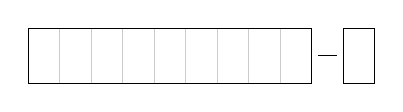
\begin{tikzpicture}[xscale=.4,yscale=.7]
    \draw[gray!40] ( 0, 0) grid      ( 9, 1);
    \draw          ( 0, 0) rectangle ( 9, 1);
    \draw          (10, 0) rectangle (11, 1);
    \draw (9 + .2, .5) -- (10 - .2, .5);
  \end{tikzpicture}%
}
\newcommand{\li}{\lstinline}
\providecommand{\pond}[1]{[{\small\textbf{#1\%}}]}

\lstdefinelanguage{py}{%
  classoffset=0,%
    morekeywords={%
      False,class,finally,is,return,None,continue,for,lambda,try,%
      True,def,from,nonlocal,while,and,del,global,not,with,print,%
      as,elif,if,or,yield,assert,else,import,pass,break,except,in,raise},%
    keywordstyle=\color{black!80}\bfseries,%
  classoffset=1,
    morekeywords={int,float,str,abs,len,raw_input,exit,range,min,max,%
      set,dict,tuple,list,bool,complex,round,sum,all,any,zip,map,filter,%
      sorted,reversed,dir,file,frozenset,open,%
      array,zeros,ones,arange,linspace,eye,diag,dot},
    keywordstyle=\color{black!50}\bfseries,%
  classoffset=0,%
  sensitive=true,%
  morecomment=[l]\#,%
  morestring=[b]',%
  morestring=[b]",%
  stringstyle=\em,%
}

\lstdefinelanguage{testcase}{%
  moredelim=[is][\bfseries]{`}{`},%
  backgroundcolor=\color{gray!20},%
}

\lstdefinelanguage{file}{%
  frame=single,%
}

\lstset{language=py}
\lstset{basicstyle=\ttfamily}
\lstset{columns=fixed}
\lstset{upquote=true}
\lstset{showstringspaces=false}
\lstset{rangeprefix=\#\ }
\lstset{includerangemarker=false}

\newlist{certamen}{enumerate}{1}
\setlist[certamen]{%
  label=\arabic*.,
  font=\LARGE\bfseries,%
  labelindent=-.5in,%
  leftmargin=0pt,%
  labelsep=1em%
}



\begin{document}

  \begin{enumerate}[font=\Large\bfseries]

    \item[1a.]
      Indique qué es lo que imprimen los siguientes programas.

      \foreach \x in {1,2} {
        \noindent
        \begin{minipage}[b]{.5\textwidth}
          \lstinputlisting{p\x.py}
          \framebox[.8\textwidth]{\rule[10ex]{0pt}{0pt}}
          \vspace{0.4em}
        \end{minipage}
      }

    \item[1b.]
      Rutee el siguiente programa
      e indique qué es lo que imprime.

      Cada vez que el valor de una variable cambie,
      ponga su valor en una nueva fila de la tabla.
      La tabla tiene filas de sobra.

      \begin{minipage}[T]{.5\textwidth}
        \lstinputlisting{ruteo.py}
        \framebox[.8\textwidth]{\rule[10ex]{0pt}{0pt}}
      \end{minipage}
      \begin{minipage}[t]{.4\textwidth}\centering
        \begin{tabular}{|p{4em}|p{4em}|p{4em}|}\hline
            \cc{a} & \cc{b} & \cc{c} \\ \hline\hline
            && \\\hline
            && \\\hline
            && \\\hline
            && \\\hline
            && \\\hline
            && \\\hline
            && \\\hline
            && \\\hline
            && \\\hline
            && \\\hline
            && \\\hline
            && \\\hline
            && \\\hline
            && \\\hline
            && \\\hline
            && \\\hline
            && \\\hline
            && \\\hline
            && \\\hline
            && \\\hline
            && \\\hline
            && \\\hline
            && \\\hline
            && \\\hline
            && \\\hline
         \end{tabular}
      \end{minipage}

    \newpage
    \item[2.]
      Los tres lados \(a\), \(b\) y \(c\) de un triángulo
      deben satisfacer la \emph{desigualdad triangular}:
      cada uno de los lados no puede ser más
      largo que la suma de los otros dos.

      Escriba un programa que reciba como entrada
      los tres lados de un triángulo, e indique:
      \begin{itemize}
        \item si acaso el triángulo es inválido
          (no satisface la desigualdad triangular);
        \item si no lo es, qué tipo de triángulo es
          (escaleno, isóceles o equilátero).
      \end{itemize}

      \begin{minipage}[t]{.40\textwidth}
        \lstinputlisting[language=testcase,frame=single]{caso2a.txt}
      \end{minipage}
      \hfil
      \begin{minipage}[t]{.40\textwidth}
        \lstinputlisting[language=testcase,frame=single]{caso2b.txt}
      \end{minipage}
      \\
      \begin{minipage}[t]{.40\textwidth}
        \lstinputlisting[language=testcase,frame=single]{caso2c.txt}
      \end{minipage}
      \hfil
      \begin{minipage}[t]{.40\textwidth}
        \lstinputlisting[language=testcase,frame=single]{caso2d.txt}
      \end{minipage}

    \newpage
    \item[3.]
      La función seno puede ser representada
      como la siguiente suma infinita:
      \[
        \text{sen}(x) =
          \frac{x^{ 1}}{{ 1}!} -
          \frac{x^{ 3}}{{ 3}!} +
          \frac{x^{ 5}}{{ 5}!} -
          \frac{x^{ 7}}{{ 7}!} +
          \frac{x^{ 9}}{{ 9}!} -
          \frac{x^{11}}{{11}!} +
          \frac{x^{13}}{{13}!} -
          \cdots,
      \]
      donde \(n! = 1\cdot 2\cdot\,\cdots\,\cdot n\)
      es el factorial de \(n\).

      Los términos de la suma son cada vez más pequeños,
      por lo que tomando algunos de los primeros términos
      es posible obtener una buena aproximación de la función.

      Escriba un programa que pregunte al usuario
      un valor de \(x\) y una precisión \(p\),
      y entregue como salida el valor aproximado de \(\text{sen}(x)\),
      obtenido al sumar términos de la suma infinita
      hasta que la diferencia entre dos sumandos consecutivos
      sea menor o igual que \(p\).

      \begin{minipage}[t]{.40\textwidth}
        \lstinputlisting[language=testcase,frame=single]{caso3.txt}
      \end{minipage}

    \newpage
    \item[4.]

      Las \emph{ecuaciones de Lotka-Volterra}
      describen cómo cambian las poblaciones de dos especies en un ecosistema,
      en el que una de ellas es depredadora de la otra.

      En un día cualquiera,
      \(y\) representa el número de depredadores (por ejemplo, lobos),
      \(x\) el número de presas (por ejemplo, conejos),
      y el cambio de estas cantidades de un día para el otro
      están dados por las ecuaciones:
      \begin{align*}
        \Delta x &\approx \phantom{-}x(\alpha - \beta  y) \\
        \Delta y &\approx           -y(\gamma - \delta x)
      \end{align*}
      donde \(\alpha\), \(\beta\), \(\gamma\) y \(\delta\)
      son parámetros que dependen de las características del ecosistema.

      Para que el modelo funcione,
      \(x\) e \(y\) deben ser tratados como números reales,
      no como enteros.

      Suponga que en un ecosistema inicialmente hay
      \(x = 300\) conejos e \(y = 400\) lobos,
      y que la dinámica del sistema es descrita por los valores
      \(\alpha = 3\cdot 10^{-2}\),
      \(\beta  = 4\cdot 10^{-5}\),
      \(\gamma = 5\cdot 10^{-2}\) y
      \(\delta = 6\cdot 10^{-6}\).

      Escriba un programa que calcule y muestre
      en cuántos días se extinguirán los conejos
      (es decir, \(y < 1\)).

      La salida debe verse así:

      \begin{minipage}[t]{.60\textwidth}
        \lstinputlisting[language=testcase,frame=single]{caso4.txt}
      \end{minipage}

  \end{enumerate}
\end{document}

